\begin{figure*}[t]
\centering
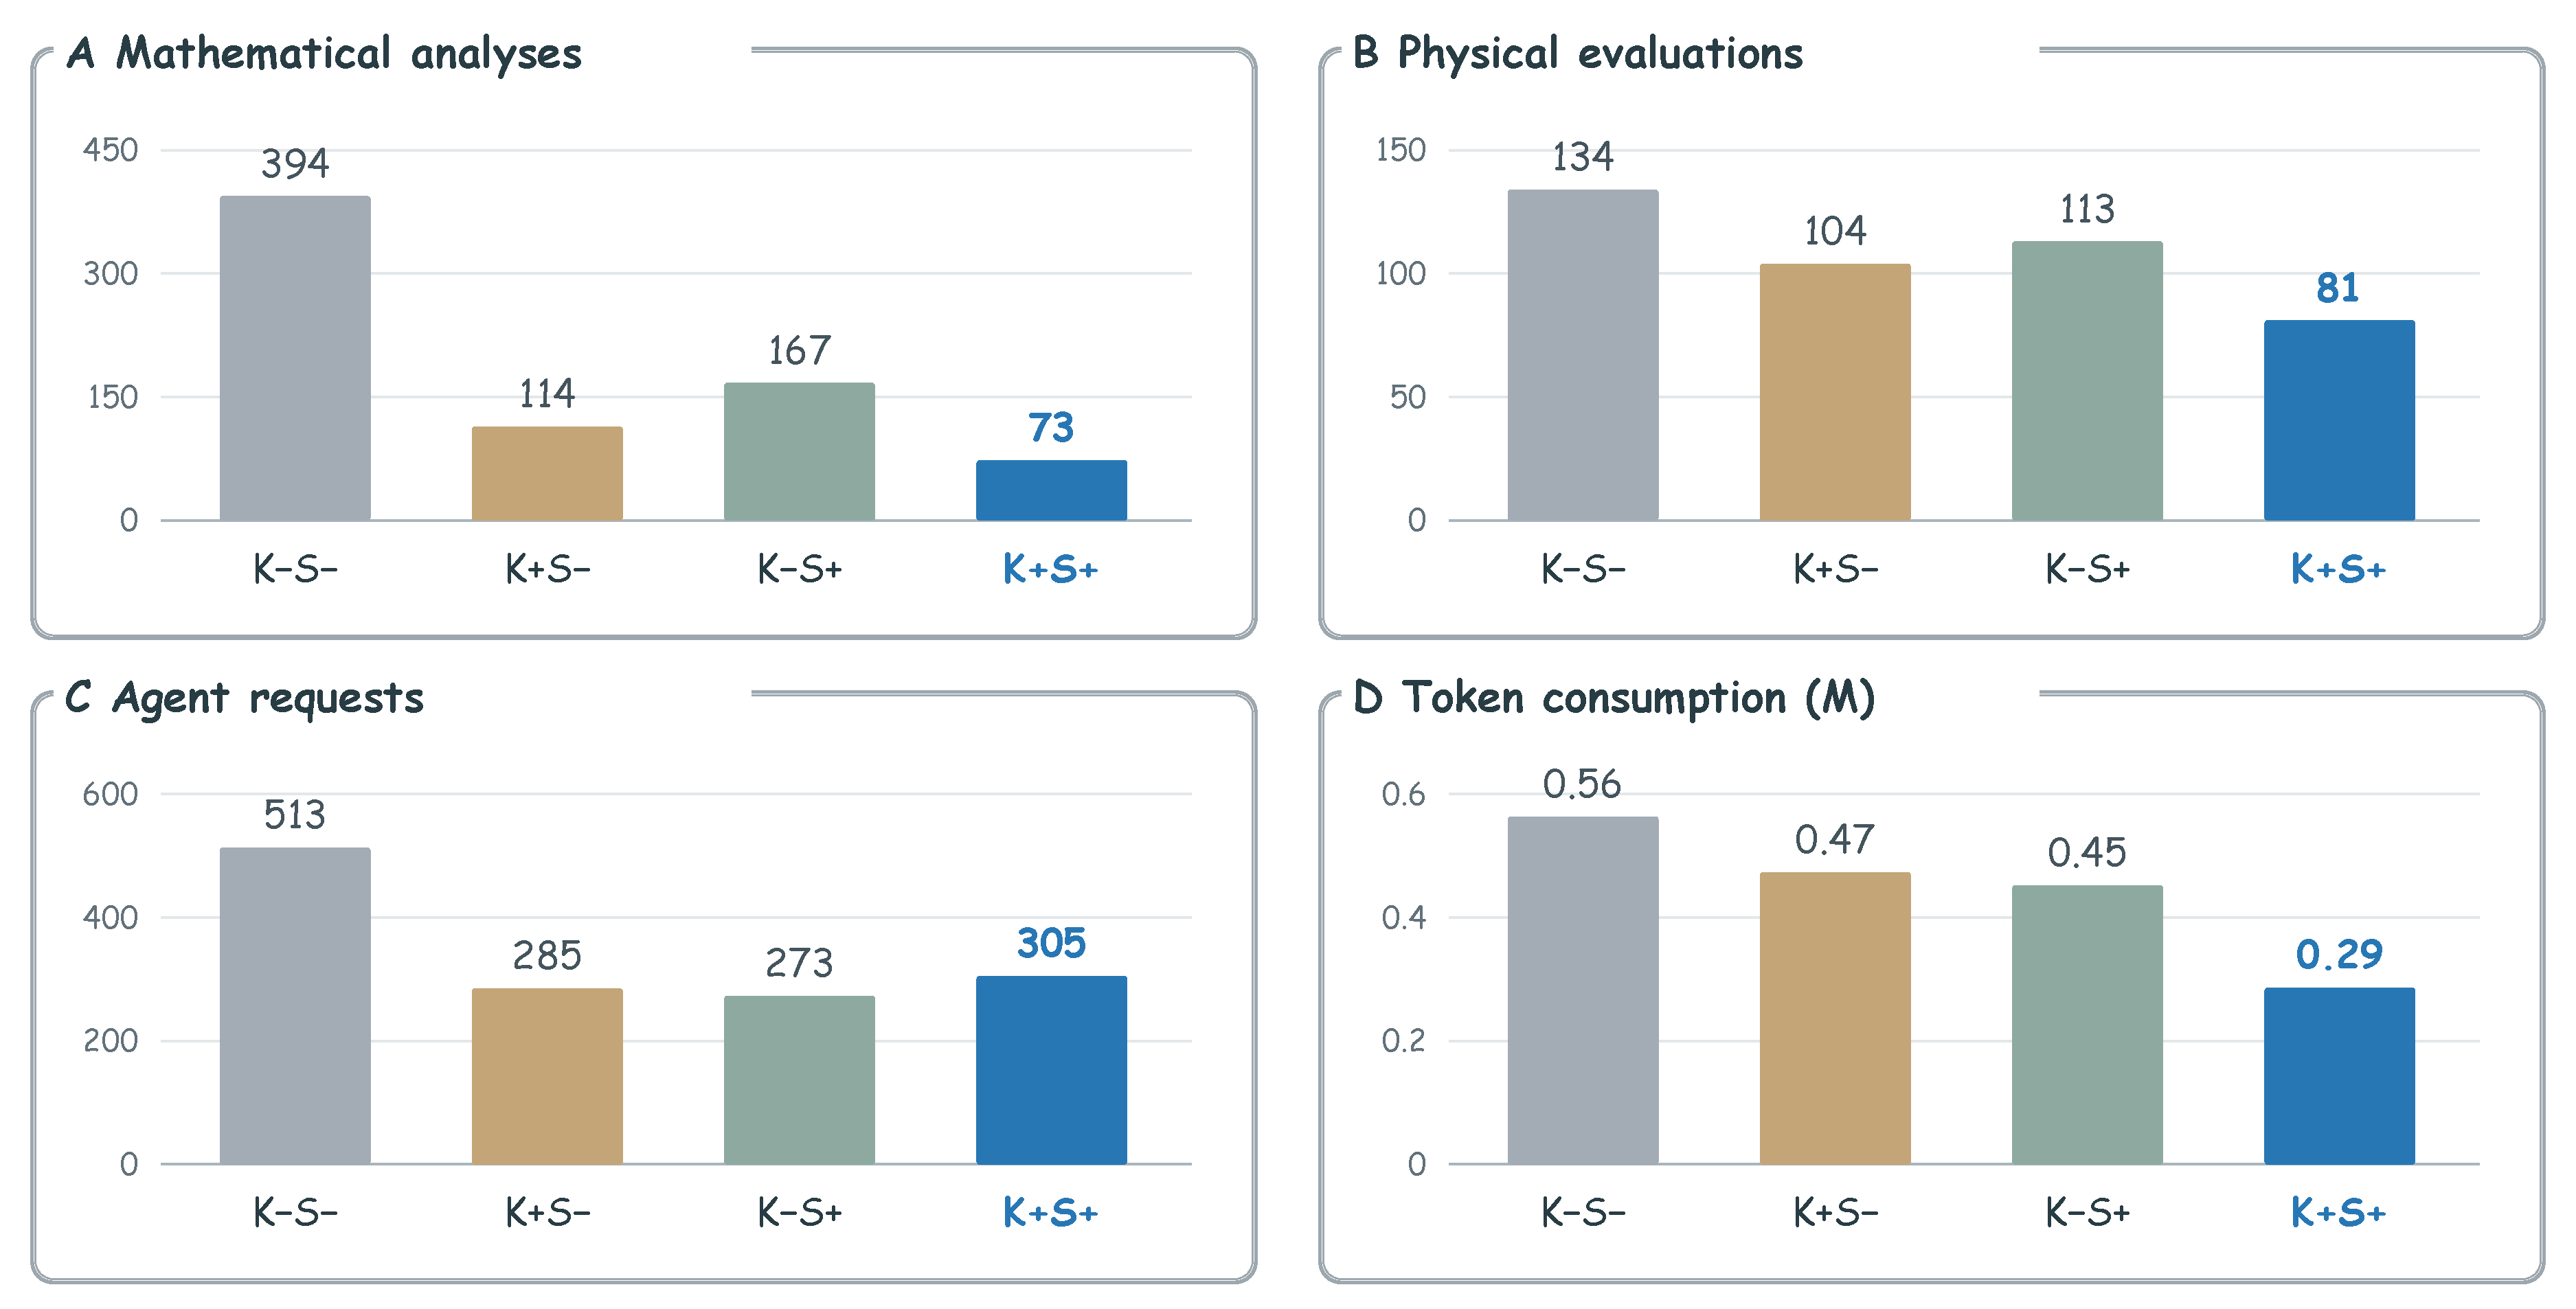
\includegraphics[width=\textwidth]{figures/fig06_knowledge_skill_resources.pdf}
\caption{Knowledge and Skill reshape research workload across eleven tasks. Each task panel separates four resource groups; within each group, bars compare K$-$S$-$, K$+$S$-$, K$-$S$+$, and K$+$S$+$ in this order. Independent min--max normalization maps the lowest recorded workload to the baseline and the highest to full height. Bar heights support comparisons only within the same task and resource group, not across tasks or resource types, and do not represent percentage savings. Equal-valued groups are marked Equal and shown at mid-height. Dark-gray crosshatching labeled NA denotes unavailable data outside the scale. Checkmarks identify configurations that complete the task. The final panel sums recorded workload over the eleven tasks before applying separate min--max normalization to each resource; its header reports completed-task counts. The K$+$S$-$ token aggregate is marked $\geq$ because only ten task records are available. Mathematical evaluations, physical launches, Core request records, and tokens follow the accounting definitions in Appendix~\ref{app:cross-model-profile}; task outcomes appear in Table~\ref{tab:abc-comparison}.}
\label{fig:knowledge-skill-resources}
\end{figure*}
